\documentclass[a4paper, 11pt]{article}
% TeX-template
% Copyright (c) 2024 Joseph Tooby-Smith. All rights reserved.
% Released under Apache 2.0 license.
% Paper content: 
% Copyright (c) 2024 Joseph Tooby-Smith. All rights reserved.
\usepackage{xcolor}
\usepackage{setspace}
\onehalfspacing%
\usepackage{bbm}
%\setstretch{3} % Custom separation of lines.
%%%%%%%%%%%%%%%%%%%%%%%%%%%%%%%%
%Hyperlinks
\usepackage{hyperref}
\definecolor{mycolor}{RGB}{0,88,204}
\hypersetup{
  colorlinks=true,
  linkcolor=mycolor,
  urlcolor=mycolor,
  citecolor=mycolor
}
%%%%%%%%%%%%%
%Watermark
\usepackage{draftwatermark}
\SetWatermarkText{\color{mycolor} DRAFT}
\SetWatermarkScale{1.5}
%%%%%%%%%%%%%%%%%%%%%%%%%%%%%%%%
%Mathematics
\usepackage{amsmath}
%%%%%%%%%%%%%%%%%%%%%%%%%%%%%%%%
%Margins
\usepackage{geometry}

\geometry{
  top=0.8in,
  bottom=0.8in,
  left=1in,
  right=1in
}
%%%%%%%%%%%%%%%%%%%%%%%%%%%%%%%%
%Page numbers
\usepackage{fancyhdr}


\pagestyle{fancy}
\fancyhf{}
\fancyhead[R]{\thepage}
\renewcommand{\headrulewidth}{0pt}
\setlength{\headheight}{13.6pt}
%For the title page
\fancypagestyle{plain}{%
  \fancyhf{}
  \fancyhead[R]{\thepage}
  \renewcommand{\headrulewidth}{0pt}
}
%%%%%%%%%%%%%%%%%%%%%%%%%%%%%%%%
%Fonts

\usepackage{mathptmx}

%%%%%%%%%%%%%%%%%%%%%%%%%%%%%%%%
%Section style

\usepackage{titlesec}

\titleformat{\section}
  {\normalfont\large\centering}{\thesection.}{1em}{\MakeUppercase}
\titleformat{\subsection}
  {\normalfont\centering}{\thesubsection.}{1em}{\MakeUppercase}

  \titlespacing{\paragraph}{10pt}{0pt}{6pt}[0pt]
%%%%%%%%%%%%%%%%%%%%%%%%%%%%%%%%
%Comments

\newcommand{\js}[1]{ {\color{magenta} js:  #1}}

%%%%%%%%%%%%%%%%%%%%%%%%%%%%%%%%
%SVG images

\usepackage{svg}
%%%%%%%%%%%%%%%%%%%%%%%%%%%%%%%%
%tikzcd
\usepackage{tikz-cd} 			
\usepackage{tikz}
\usetikzlibrary{arrows.meta}
%%%%%%%%%%%%%%%%%%%%%%%%%%%%%%%%
%Paragraph markers
%\newcommand{\paragraphMarker}[1]{ %{\color{gray} $\langle$#1$\rangle$}
%}
%%%%%%%%%%%%%%%%%%%%%%%%%%%%%%%
%Lean formating
\usepackage{listings}
\usepackage[T1]{fontenc}
\usepackage[utf8]{inputenc}
\usepackage{amssymb}
\usepackage{chngcntr}
\definecolor{keywordcolor}{rgb}{0.7, 0.1, 0.1}   % red
\definecolor{tacticcolor}{rgb}{0.0, 0.1, 0.6}    % blue
\definecolor{commentcolor}{rgb}{0.4, 0.4, 0.4}   % grey
\definecolor{symbolcolor}{rgb}{0.0, 0.1, 0.6}    % blue
\definecolor{sortcolor}{rgb}{0.1, 0.5, 0.1}      % green
\definecolor{attributecolor}{rgb}{0.7, 0.1, 0.1} % red

\def\lstlanguagefiles{lstlean.tex}
\lstset{
 	frame = lrtb,
 	rulecolor=\color{mycolor},
	language=lean,
	aboveskip = 5mm,
	belowskip = 5mm,
	captionpos=t
	}

\lstnewenvironment{code}[1][]%
{
   \noindent\newline
   \minipage{\linewidth}
   \vspace{0.5\baselineskip}
   \lstset{
 	frame = lrtb,
 	rulecolor=\color{mycolor},
 	escapeinside={/*!}{!*/},
	language=lean,
	aboveskip = 5mm,
	belowskip = 5mm,
	xleftmargin=2mm,
	xrightmargin=2mm,
	}
	}
{\endminipage\newline}
\lstnewenvironment{codeLong}[1][]%
{
   \lstset{
 	frame = lrtb,
 	rulecolor=\color{mycolor},
 	escapeinside={/*!}{!*/},
	language=lean,
	aboveskip = 5mm,
	belowskip = 5mm,
	xleftmargin=2mm,
	xrightmargin=2mm,
	}
	}
{}
%%%%%%%%%%%%%%%%%%%%%%%%%%%%%%%%
%Links in code block
% put at top of code block using
% /*!\codeLink{...}!*/
\newcommand{\codeLink}[1]{
  \vspace{-0.5cm}\hfill\href{https://github.com/HEPLean/HepLean/blob/1b951994ae3d882242b02d23957ef1ee7fa05f3d/HepLean/#1}{(source)}
  }
  \newcommand{\codeBreakdownLink}[2]{
  \vspace{-0.5cm}\hfill\href{https://github.com/HEPLean/HepLean/blob/1b951994ae3d882242b02d23957ef1ee7fa05f3d/HepLean/#1}{(source)}
  (breakdown \ref{#2})
  }
 \newcommand{\textLink}[1]{\href{https://github.com/HEPLean/HepLean/blob/1b951994ae3d882242b02d23957ef1ee7fa05f3d/HepLean/#1}{source}}
 \newcommand{\textLinkB}[1]{\href{https://github.com/HEPLean/HepLean/blob/1b951994ae3d882242b02d23957ef1ee7fa05f3d/HepLean/#1}{(source)}}

%%%%%%%%%%%%%%%%%%%%%%%%%%%%%%%%
% Syntax elab code block 
\usepackage[table]{xcolor}
\newcommand{\syntaxElab}[2]{ 
  \arrayrulecolor{mycolor}
  \begin{center}
    \begin{tabular}{|p{1.7in} | p{4in}|}
    \hline
    \hfill {#1} & {#2} \\
    \hline
    \end{tabular}
    \end{center}
  \arrayrulecolor{black}
}
%%%%%%%%%%%%%%%%%%%%%%%%%%%%%%%%
%Proof step 

\newcommand{\proofstep}[3]{
  \arrayrulecolor{mycolor}
\begin{center}
\begin{tabular}{|p{3in}| p{3in}|}
\hline
{#1
}\newline 
\hrule~\newline
#2
  & ~\newline
\makebox[3in]{%
#3}
  \\ \hline
\end{tabular}
\end{center}
\arrayrulecolor{black}
}
%%%%%%%%%%%%%%%%%%%%%%%%%%%%%%%%
%Math commands 
\newcommand{\Rep}[2]{\mathrm{Rep} \; #1 \; #2}
%%%%%%%%%%%%%%%%%%%%%%%%%%%%%%%%
%Title, author, date
\title{Index notation in Lean 4}
\author{Joseph Tooby-Smith \\ \textit{Reykjavik University}}
\date{\today}
%%%%%%%%%%%%%%%%%%%%%%%%%%%%%%%%

\begin{document}
\counterwithin{lstlisting}{section}
\maketitle
\vspace{-1cm}
\begin{abstract}
The physics community relies on index notation to effectively manipulate tensors of specific 
types. This paper introduces the first formally verified implementation of index notation in the
interactive theorem prover Lean 4. By integrating index notation into Lean, we bridge the gap between 
traditional physics notation and formal verification tools, 
making it more accessible for physicists to write and prove results within Lean.
In the background, our implementation leverages a novel application of category theory.
\end{abstract}

\section{Introduction}

In previous work, the author initiated the digitalization (or formalization) 
of high energy physics 
results using the interactive theorem prover Lean 4 in a project called HepLean. 
Lean is a
programming language with syntax resembling traditional pen-and-paper mathematics. 
Users can write definitions, theorems, and proofs in Lean,
which are then automatically checked using dependent-type theory for correctness.
The HepLean project is driven by four primary motivations: to facilitate easier look-up of results
 through linear information storage; to support the creation and proof of new results using 
 automated tactics and AI tools; to facilitate correctness checking of result in high energy physics; 
 and to introduce new pedogocial methods for high-energy physics and computer science.

HepLean is part of a broader movement of projects
to formalize parts, or all, of 
mathematics and science. The largest of these projects is Mathlib, which aims to formalize
mathematics. Indeed, HepLean is built downstream of Mathlib, meaning it has Mathlib as a 
dependency and uses many of the definitions and theorems thereof. 
Other projects include the ongoing effort led by Kevin Buzzard to formalize the proof of Fermat's
Last Theorem into Lean. 
In the realm of the sciences, the paper~\cite{josephson} looks at absorption theory, thermodynamics, and kinematics in Lean. 
Whilst the package SciLean~\cite{SciLean}, is a push in the direction of scientific computing within Lean. 

Physicists heavily rely on specialized notation to express mathematical concepts succinctly. 
Among these, index notation is particularly prevalent,
 as it provides a compact and readable way to represent specfic types of tensors and operations
 between them, with tensors forming a backbone of morden physics. 

Because of the importance of index notation, it is crucial to have a way to write index notation in Lean. 
This will make results from high energy physics easier to write and prove in Lean. 
Additionally, it will make the syntax more familiar to high energy physicists.
Such an implementation is the subject of this paper. 
It is a challange because, not only do we need an implentation that is nice and flexiable to use, 
we also need it to be formally well-defined and rigourous. 
We hope that the implementation presneted here will
not only enhances usability of Lean but also promotes the adoption of formal methods in the 
physics community.


As a taster of what is to come, our implmentation allows to write results like the following in 
Lean:
\begin{code}
{pauliCo | ν α β ⊗ pauliContr | ν α' β' = 2 •ₜ εL | α α' ⊗ εR | β β'}ᵀ
\end{code}
Lean will correctly interpret this result as a tensor expression which the correct contraction of indices 
and permutation of indices between the sides of the expression.

Previous implmentations of index notation have been made in programming languages like Haskell 
\cite{ref}. However, these implementations do not
 provide the formal verification capabilities inherent in Lean. 
 The formal verification requirement of Lean introduces unique challenges in implementing index 
 notation, necessitating (what we beleive is) a novel solution.


This paper is split into two main sections. Section~\ref{sec:Implementation} dicusses 
the implementation of index notation into Lean. Section \js{ref} gives two examples 
of theorems and proofs using index notation. A more minor section, section \js{ref} disucsses 
the future work related to this project.


\section{Implementation of index notation into Lean 4}\label{sec:Implementation}
\begin{figure}
  \centering
  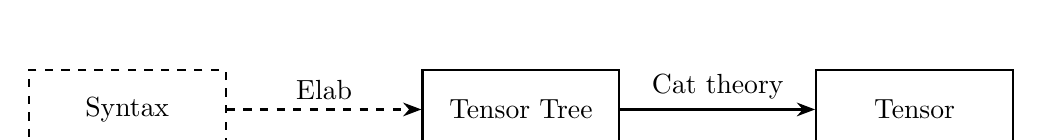
\begin{tikzpicture}[
    thick,
    >=Stealth,
    box/.style={rectangle, draw, minimum height=1cm, minimum width=2.5cm, align=center},
    dashedbox/.style={rectangle, draw, dashed, minimum height=1cm, minimum width=2.5cm, align=center}
  ]
  
  % Nodes
  \node[dashedbox] (syntax) at (0,0) {Syntax};
  \node[box] (tensorTree) at (5,0) {Tensor Tree};
  \node[box] (tensor) at (10,0) {Tensor};
  
  % Edges
  \draw[->, dashed] (syntax) -- node[above] {Elab} (tensorTree);
  \draw[->] (tensorTree) -- node[above] {Cat theory} (tensor);
  
  \end{tikzpicture}
  \caption{Overview of the implementation of index notation in Lean. The 
  solid lines represent formally verified parts of the implementation.}
  \label{fig:overviewFlow}
\end{figure}
Our implementation of index notation in Lean can be  broken down into 
three main components, illustrated in Figure~\ref{fig:overviewFlow}. 
The first component is the \emph{syntax for tensor expressions}, 
which is what users interact with when writing results in Lean. 
This syntax closely mirrors the notation familiar to physicists, 
making it intuitive and accessible. 
It appears directly in the Lean files and can be thought of as an informal string 
that represents the tensor expressions. The code snippet above, involving pauli matrices, is an 
example of this.

The second component involves transforming this syntax into a \emph{tensor tree}. 
The tensor tree is a formal mathematical representation of the tensor expression. 
By parsing the syntax into a structured tree, 
we establish a rigorous foundation that captures the tensor expression. 
This formal representation allows us to easily manipulate tensor expressions and
prove results related to them in a way that Lean accepts as formal.

The third and final component is the conversion of the tensor tree into an actual \emph{tensor}. 
This process utilizes properties of the symmetric-monoidal category of representations
 to translate the tensor tree into a tensor.

Although Lean processes information from left to right in Figure~\ref{fig:overviewFlow}, 
starting with the syntax and proceeding to the tensor tree, and then finally (when 
we ask it to) to the tensors, 
it is more effective to discuss the implementation from right to left. 
Starting with tensors is advantageous because they are the primary objects of interest.
 The left and middle parts of the diagram can be thought of as intermediate stages that facilitate the 
 manipulation and understanding of these tensors and their expressions.

\subsection{Defining tensors} \label{sec:definingTensors}

\subsubsection{Building blocks of tensors and color} \label{sec:buildingBlocks}

Tensors of a species, such as complex Lorentz tensors, are constructed from a 
set of building block representations of a group $G$ over a field $k$.

For complex Lorentz tensors, the group $G$ is $SL(2, \mathbb{C})$, the field $k$ is the 
field of complex numbers and six building block representations. The six building block representations 
are
\begin{itemize}
  \item The representation of left-handed Weyl fermions, 
    denoted in Lean as \lstinline|Fermion.leftHanded|, and corresponding to the 
    representation of $SL(2, \mathbb{C})$ taking $v \mapsto M v$ for $M \in SL(2, \mathbb{C})$.
  \item The representation of `alternative' left-handed Weyl fermions, 
    denoted in Lean as \lstinline|Fermion.altLeftHanded|, and corresponding to the 
    representation of $SL(2, \mathbb{C})$ taking $v \mapsto M^{-1 T} v$ for $M \in SL(2, \mathbb{C})$.
  \item The representation of right-handed Weyl fermions, 
    denoted in Lean as \lstinline|Fermion.rightHanded|, and corresponding to the 
    representation of $SL(2, \mathbb{C})$ taking $v \mapsto M^\star v$ for $M \in SL(2, \mathbb{C})$.
  \item The representation of `alternative' right-handed Weyl fermions,
    denoted in Lean as \lstinline|Fermion.altRightHanded|, and corresponding to the 
    representation of $SL(2, \mathbb{C})$ taking $v \mapsto M^{-1 \dagger} v$ for $M \in SL(2, \mathbb{C})$.
  \item The representation of contravariant Lorentz tensors, 
    denoted in Lean as \lstinline|Lorentz.complexContr|, and corresponding to the 
    representation of $SL(2, \mathbb{C})$ induced by the homomorphism of $SL(2, \mathbb{C})$ into 
    the Lorentz group and the contravariant action of the Lorentz group on four-vectors.
  \item The representation of covariant Lorentz tensors,
     denoted in Lean as \lstinline|Lorentz.complexCo|, and corresponding to the 
    representation of $SL(2, \mathbb{C})$ induced by the homomorphism of $SL(2, \mathbb{C})$ into 
    the Lorentz group and the covariant action of the Lorentz group on four-vectors.
\end{itemize}
As an example the representation \lstinline|Fermion.leftHanded| is defined in Lean as follows:
\begin{codeLong}
/-- The vector space ℂ^2 carrying the fundamental representation of SL(2,C).
  In index notation corresponds to a Weyl fermion with indices ψ^a. -/
def leftHanded : Rep ℂ SL(2,ℂ) := Rep.of {
  /- The function from SL(2,ℂ) to endomorphisms of LeftHandedModule 
    (which corresponds to the vector space ℂ^2). -/
  toFun := fun M => {
    /- Start of the definiton of the linear map. -/
    /- The function underlying the linear map. Defined as the dot product. -/
    toFun := fun (ψ : LeftHandedModule) =>
      LeftHandedModule.toFin2ℂEquiv.symm (M.1 *ᵥ ψ.toFin2ℂ),
    /- Proof that the function is linear with respect to addition. -/
    map_add' := by
      intro ψ ψ'
      simp [mulVec_add]
    /- Proof that the function is linear with respect to scalar multiplication. -/
    map_smul' := by
      intro r ψ
      simp [mulVec_smul]
    /- End of the definiton of the linear map. -/}
  /- Proof that (the outer) toFun gives the identity map on the identity of SL(2,ℂ). -/
  map_one' := by
    ext i
    simp
  /- Proof that the action of the product of two elements is 
    the product of the actions of the elements. -/
  map_mul' := fun M N => by
    simp only [SpecialLinearGroup.coe_mul]
    ext1 x
    simp only [LinearMap.coe_mk, AddHom.coe_mk, LinearMap.mul_apply, LinearEquiv.apply_symm_apply,
      mulVec_mulVec]}
\end{codeLong} 
We have added some explainatory comments to this code, not seen in the actual Lean code, to give 
the reader an idea of what each part does. 

We assign a unique label, which we refer to as a \emph{color}, to each of the 
building block representations. We denote the type of colors for a given species of tensors as $C$.
For complex Lorentz tensors 
$C$ is defined as 
\begin{code}
inductive Color
  | upL : Color
  | downL : Color
  | upR : Color
  | downR : Color
  | up : Color
  | down : Color
\end{code}
Here \lstinline|Color| is the name of our type and \lstinline|upL|, \lstinline|downL|, etc. are the
colors. 

To formally associate each color with its corresponding representation, we define
a discrete functor from the set $C$ to the category of $k$-representations of $G$, denoted 
$\Rep k G$, that is, a functor
\begin{equation} 
  F_{D} : C \Rightarrow \Rep k G
\end{equation}


For complex Lorentz tensors this functor in Lean as follows:
\begin{code}
FDiscrete := Discrete.functor fun c =>
  match c with
  | Color.upL => Fermion.leftHanded
  | Color.downL => Fermion.altLeftHanded
  | Color.upR => Fermion.rightHanded
  | Color.downR => Fermion.altRightHanded
  | Color.up => Lorentz.complexContr
  | Color.down => Lorentz.complexCo
\end{code}

The reason why we have used a functor here, rather than just a function, will become apparent
in what follows.


\subsubsection{General tensors} \label{sec:generalTensors}

For a given tensor species, given the symmetric monoidal structure on $\mathrm{Rep} k G$, 
we can take the tensor product of the building block representations. 
Elements of such tensor products form the general notion of a tensor for that given 
species. 

To formalize this in Lean, we consider the category  $\mathcal{S}_{/C}^\times$. The objects 
of $\mathcal{S}_{/C}^\times$ are functions $f : X \to C$  for some type $X$. 
A morphism from $f : X \to C$ to $g : Y \to C$ is a bijection $\phi : X \to Y$ such that 
$f = g \circ \phi$. 
This category is equivalent to the core of the category of types ($\mathcal{s}$) over $C$, hence 
our notation. 

Any functor $H : C \Rightarrow \mathrm{Rep} k G$ can be lifted to a symmetric monoidal 
functor $\mathcal{S}_{/C}^\times \Rightarrow \mathrm{Rep} k G$ which takes $f$ to the 
tensor product $\bigotimes_{x \in X} H(f(x))$ and morphisms to the linear maps 
of representations corresponding to reindexings of
tensor products.

This construction is itself functorial, 
giving a functor: 
\begin{equation}
  \mathrm{lift} : \mathrm{Fun}(C, \mathrm{Rep} k G) \Rightarrow
  \mathrm{SymmMonFun}(\mathcal{S}_{/C}^\times, \mathrm{Rep} k G)
\end{equation} 
In the previous subsection we defined the functor $F_{D}$ which associates to each color 
its corresponding representation. We can then define a functor $F$ by the image of $F_{D}$ under
the lift functor. 

A tensor of a given species can then be thought of as a vector in the representations in the of $F$.
Defining a tensor in this way allows us to utalize the 
structur of monodial categories and functors in a useful way. 

In HepLean we formally define $\mathrm{lift}$ and $F$. 

For most purposes in physics $X$ will be a type $\mathrm{Fin} n$, corresponding to the type 
(set) of natural numbers (including 0) less $n$. Later on we will restrict to these types.

\subsubsection{Tensor operations} \label{sec:tensorOperations}

Now we have discussed how tensors of a given species can be formally defined, we can define 
basic operations on these tensors. 


The simipalist of these operations are addition, scalar multiplication and group action.
Addition and scalar multiplication are given to us for free from the vector space structure 
on $F(f)$. The action of the group $G$ on tensors also comes for free from the fact that 
$F(f)$ lives in $\mathrm{Rep} k G$.

The next simplest operation is permutation of indices (or building block representations).
Such permutations arise from applying $F$ to morphisms in $\mathcal{S}_{/C}^\times$. 
Theses sorts of permutations are often implicit in the notation physicists use, but arise 
in tensor expressions such as $T_{\mu \nu} = T_{\nu \mu}$.

The next operation is the tensor product of two tensors. Given $f : X \to C$ and
$g : Y \to C$, and tensors $t \in F(f)$ and $s \in F(g)$ we can form a vector in 
$F(f) \otimes F(g)$. Formally this can be done by taking the tensor product of the morphisms
$\mathbbm{1} \to F(f)$ and $\mathbbm{1} \to F(g)$ in the category of vector spaces over $k$.
We can then use the tensorate of $F$ to get a tensor in $F(f \otimes g)$.

We now turn to the slightly more complicated operation of contraction of indices, 
and the related metric and unit. 
To define the contraction of introduce an involution $\tau : C \to C$. For complex Lorentz tensors
this is defined as follows
\begin{code} 
  τ := fun c =>
    match c with
    | Color.upL => Color.downL
    | Color.downL => Color.upL
    | Color.upR => Color.downR
    | Color.downR => Color.upR
    | Color.up => Color.down
    | Color.down => Color.up
\end{code}
We say that $\tau$ takes a color to it's dual. With $\tau$ and $F_D$ we can define 
the functor  $F_\tau : C \Rightarrow Rep k G$ which takes $c$ to $F(c) \otimes F(\tau c)$. 
Letting $\mathbbm{1}$ be the constant functor from $C$ landing on the, we basic data 
for contraction is contained in a natural transformation from $F_\tau$ to $\mathbbm{1}$.
That is, for each $c \in C$ an equivariant map from $F(c) \otimes F(\tau c)$ to the trivial 
representation. 

To see how this is can be used to contract indices, consider a tensor $t \in F(f)$, 
for $f : \mathrm{Fin} \; n.succ.succ \to C$. Here $\mathrm{Fin} \; n.succ.succ$ is the type 
of all number ${0, 1, 2, \ldots, n+1}$ less than $n.succ.succ = n + 2$. 
Choosing two distinct indices $i, j : \mathrm{Fin} \; n.succ.succ$ we can contract them 
using the following chain of maps
\begin{equation}
  F f \equiv F_\tau (f i) \otimes F (f' i) \to \mathbbm{1} \otimes F (f' i) \to F (f' i)
\end{equation}
Here $f' : \mathrm{Fin} \; n \to C$ is the function defived from $f$ by removing the indices $i$ 
and $j$. The first equivalence is somewhat complicated to define formally, but essentially involves 
extracting $i$ and $j$. 

The metric and unit are defined in a similar way. The metric is a natural transformation from
$\mathbbm{1}$ to $F_D\otimes F_D$. That is, for each $c \in C$ an equivariant map from the trivial
representation to $F_D(c) \otimes F_D(c)$. The unit is a natural transformation from $\mathbbm{1}$ to
$F_\tau'$ which takes $c$ to $F_D(\tau c) \otimes F_D(c)$. That is, for each $c \in C$ an 
equivariant map from the trivial representation to  $F_D(\tau c) \otimes F_D(c)$.

The choice of contraction, metric and unit are subject to a number of conditions.
\begin{itemize}
\item Contraction must be symmetric.
\begin{equation}
  \begin{tikzcd}
    F_D(c) \otimes F_D(\tau c) \arrow[r, "{\beta}"] \arrow[d, "{\mathcal{C}\, c}", swap] & F_D(\tau c) \otimes F_D (c) \arrow[d, "\mathbbm{1} \otimes F_D t"] \\
    \mathbb{I} & F_D(\tau c) \otimes F_D (\tau \tau c) \arrow[l, "{\mathcal{C}\, \tau(c)}", ] 
  \end{tikzcd}
  \end{equation}
  \item Contraction with the unit does nothing. 
  \begin{equation}
    \begin{tikzcd}
      F_D(c) \arrow[r] &  F_D(c) \otimes \mathbb{I} \arrow[r] & F_D(c) \otimes (F_D (\tau c) \otimes F_D(c)) \arrow[d] \\
      \mathbb{I} \otimes F_D(c) \arrow[u] &   &(F_D(c) \otimes F_D(\tau c)) \otimes F_D(c) \arrow[ll] 
  \end{tikzcd}
  \end{equation}
  \item The unit is symmetric 
  \begin{equation} 
    \begin{tikzcd}
      \mathbb{I} \arrow[r] \arrow[d] & F_D(\tau c) \otimes F_D(c) \\
      F_D(\tau \tau c) \otimes F_D(\tau c) \arrow[r] & F_D(\tau c) \otimes F_D(\tau \tau c) \arrow[u]
    \end{tikzcd}
  \end{equation}
  \item Contraction with the metric its dual returns the unit
  \begin{equation}
    \begin{tikzcd}
      \mathbb{I} \arrow[r] \arrow[d] & F_D(\tau c) \otimes F_D (c) \\ 
      (F_D c \otimes F_d c) \otimes (F_D (\tau c) \otimes F_D (\tau c) ) \arrow [d]  & F_D (c) \otimes F_D(\tau c) \arrow[u] \\ 
      F_D c \otimes (F_d c \otimes (F_D (\tau c) \otimes F_D (\tau c) )) \arrow [r] &  F_D c \otimes ((F_d c \otimes F_D (\tau c)) \otimes F_D (\tau c) ) \arrow[u]
    \end{tikzcd}
  \end{equation}
\end{itemize}
In Lean we quite write these conditions in this way, instead we give them in a simpiler equivalent form 
in which we apply the maps in the above diagram to pure tensors. We will see how they are 
written explicitly in Lean when we come to formally define the tensor species in the next section.

The last operation we want to talk about is evaluation. Where one specifies the exact value of 
one of the indices of a tensor e.g. $\eta_{0i}$. 
All of the operations disucsed thus far have related to the category $\mathrm{Rep} k G$. As such, 
they have respect the group action. Evaluation, on the other hand, does not respect the group action. 
For example, taking the $0$th component of a four-vector is not Lorentz invariant. 
Nevertheless, we can define evaluation in the categor of vector spaces. 
To do this, we need a basis for each $F_D(c)$, the coordinates of a vector in $F_D(c)$ in that basis 
is discrbed by a linear map of vector spaces from $F_D(c)$ to $k$. This can be used 
to evaluate the index of a tensor in the following way: 
\begin{equation} 
  F f \equiv F_D (f i) \otimes F (f' i) \to \mathbbm{1} \otimes F (f' i) \to F (f' i)
\end{equation}
where $f'$ is $f$ with the $i$th index removed, and again the first equivalence is somewhat
complicated to define but involves extracting the $i$th index.

\subsubsection{Tensor Species} \label{sec:tensorSpecies}

The data of the field $k$, the group $G$, the functor $F_D$ (from which $F$ can be derived), the involution $\tau$, the natural
transformations for contraction, metric, and unit, and basis needed for evaluation, 
form formally what we have lossely been calling a Tensor species.

That is, the difference between complex Lorentz tensors, Einstien tensors, and real Lorentz tensors 
is down to this data. 
In Lean it useful to work with general tensor species where possible, so important results have 
to be defined only ones. Thus we make the following definition 
\begin{codeLong}
/-- The sturcture of a type of tensors e.g. Lorentz tensors, Einstien tensors,
  complex Lorentz tensors. -/
structure TensorSpecies where
  /-- The colors of indices e.g. up or down. -/
  C : Type
  /-- The symmetry group acting on these tensor e.g. the Lorentz group or SL(2,ℂ). -/
  G : Type
  /-- An instance of `G` as a group. -/
  G_group : Group G
  /-- The field over which we want to consider the tensors to live in, usually `ℝ` or `ℂ`. -/
  k : Type
  /-- An instance of `k` as a commutative ring. -/
  k_commRing : CommRing k
  /-- A `MonoidalFunctor` from `OverColor C` giving the rep corresponding to a map of colors
    `X → C`. -/
  FDiscrete : Discrete C ⥤ Rep k G
  /-- A map from `C` to `C`. An involution. -/
  τ : C → C
  /-- The condition that `τ` is an involution. -/
  τ_involution : Function.Involutive τ
  /-- The natural transformation describing contraction. -/
  contr : OverColor.Discrete.pairτ FDiscrete τ ⟶ 𝟙_ (Discrete C ⥤ Rep k G)
  /-- The natural transformation describing the metric. -/
  metric : 𝟙_ (Discrete C ⥤ Rep k G) ⟶ OverColor.Discrete.pair FDiscrete
  /-- The natural transformation describing the unit. -/
  unit : 𝟙_ (Discrete C ⥤ Rep k G) ⟶ OverColor.Discrete.τPair FDiscrete τ
  /-- A specification of the dimension of each color in C. This will be used for explicit
    evaluation of tensors. -/
  repDim : C → ℕ
  /-- repDim is not zero for any color. This allows casting of `ℕ` to `Fin (S.repDim c)`. -/
  repDim_neZero (c : C) : NeZero (repDim c)
  /-- A basis for each Module, determined by the evaluation map. -/
  basis : (c : C) → Basis (Fin (repDim c)) k (FDiscrete.obj (Discrete.mk c)).V
  /-- Contraction is symmetric with respect to duals. -/
  contr_tmul_symm (c : C) (x : FDiscrete.obj (Discrete.mk c))
      (y : FDiscrete.obj (Discrete.mk (τ c))) :
    (contr.app (Discrete.mk c)).hom (x ⊗ₜ[k] y) = (contr.app (Discrete.mk (τ c))).hom
      (y ⊗ₜ (FDiscrete.map (Discrete.eqToHom (τ_involution c).symm)).hom x)
  /-- Contraction with unit leaves invariant. -/
  contr_unit (c : C) (x : FDiscrete.obj (Discrete.mk (c))) :
    (λ_ (FDiscrete.obj (Discrete.mk (c)))).hom.hom
    (((contr.app (Discrete.mk c)) ▷ (FDiscrete.obj (Discrete.mk (c)))).hom
    ((α_ _ _ (FDiscrete.obj (Discrete.mk (c)))).inv.hom
    (x ⊗ₜ[k] (unit.app (Discrete.mk c)).hom (1 : k)))) = x
  /-- The unit is symmetric. -/
  unit_symm (c : C) :
    ((unit.app (Discrete.mk c)).hom (1 : k)) =
    ((FDiscrete.obj (Discrete.mk (τ (c)))) ◁
      (FDiscrete.map (Discrete.eqToHom (τ_involution c)))).hom
    ((β_ (FDiscrete.obj (Discrete.mk (τ (τ c)))) (FDiscrete.obj (Discrete.mk (τ (c))))).hom.hom
    ((unit.app (Discrete.mk (τ c))).hom (1 : k)))
  /-- On contracting metrics we get back the unit. -/
  contr_metric (c : C) :
    (β_ (FDiscrete.obj (Discrete.mk c)) (FDiscrete.obj (Discrete.mk (τ c)))).hom.hom
    (((FDiscrete.obj (Discrete.mk c)) ◁ (λ_ (FDiscrete.obj (Discrete.mk (τ c)))).hom).hom
    (((FDiscrete.obj (Discrete.mk c)) ◁ ((contr.app (Discrete.mk c)) ▷
    (FDiscrete.obj (Discrete.mk (τ c))))).hom
    (((FDiscrete.obj (Discrete.mk c)) ◁ (α_ (FDiscrete.obj (Discrete.mk (c)))
      (FDiscrete.obj (Discrete.mk (τ c))) (FDiscrete.obj (Discrete.mk (τ c)))).inv).hom
    ((α_ (FDiscrete.obj (Discrete.mk (c))) (FDiscrete.obj (Discrete.mk (c)))
      (FDiscrete.obj (Discrete.mk (τ c)) ⊗ FDiscrete.obj (Discrete.mk (τ c)))).hom.hom
    ((metric.app (Discrete.mk c)).hom (1 : k) ⊗ₜ[k]
      (metric.app (Discrete.mk (τ c))).hom (1 : k))))))
    = (unit.app (Discrete.mk c)).hom (1 : k)
\end{codeLong}

We can then let e.g. \lstinline|S : TensorSpecies| and recover the functor $F_D$ 
by \lstinline|S.FDiscrete|. The functor $F$ is defined seperatrly can can be recovered
by \lstinline|S.F|. If \lstinline|f : X \to S.C| is map then a tensor is an element of 
\lstinline|S.F.obj (OverColor.mk f)|. The \lstinline|OverColor.mk| tells Lean to consider $f$ as 
a function an element of the category $\mathcal{S}_{/C}^\times$, or as it is written in Lean 
\lstinline|OverColor S.C|. 

A function \lstinline|f : Fin 2 → S.C|, for instance landding on $c1, c2 \in C$ can be written in 
Lean as \lstinline|![c1, c2]|, thus we can write \lstinline|S.F.obj (OverColor.mk ![c1, c2])|. 

We will see instances of this for Complex Lorentz tensors. As an example, a Lorentz tensor 
$T^\mu_\nu$ can be written as 
\begin{code}
T : complexLorentzTensor.F.obj (OverColor.mk ![Color.up, Color.down])
\end{code}

\subsection{Tensor trees} \label{sec:tensorTrees}
A tensor expression consists of a series of tensors and operations between them. 
For example 
\begin{equation}
  \eta_{\mu \nu}P^\nu_\sigma+ V_{\mu \sigma},
\end{equation}
consists of a product of tensors, a contraction and a addition. 
Such an expression is a tensor in its own right, and we could just use the operations discussed above 
to define it. 

However, it is useful for bridging the gap between syntax and a tensor to have a more structured way 
of representing such expressions.
This is where tensor trees come in. Tensor trees will also be useful when it comes to proving 
results about tensors. 

A tensor tree is essentially a tree with nodes representing tensors or operations on tensors.
For example the tensor tree for the expression above is: 

Since we really only care about tensors with $X = Fin n$, tensor trees in Lean are 
    implemented only for these. 

In Lean we define a tensor tree as follows: 
\begin{codeLong}
/-- A syntax tree for tensor expressions. -/
inductive TensorTree (S : TensorSpecies) : {n : ℕ} → (Fin n → S.C) → Type where
  /-- A general tensor node. -/
  | tensorNode {n : ℕ} {c : Fin n → S.C} (T : S.F.obj (OverColor.mk c)) : TensorTree S c
  /-- A node corresponding to the addition of two tensors. -/
  | add {n : ℕ} {c : Fin n → S.C} : TensorTree S c → TensorTree S c → TensorTree S c
  /-- A node corresponding to the permutation of indices of a tensor. -/
  | perm {n m : ℕ} {c : Fin n → S.C} {c1 : Fin m → S.C}
      (σ : (OverColor.mk c) ⟶ (OverColor.mk c1)) (t : TensorTree S c) : TensorTree S c1
  /-- A node corresponding to the product of two tensors. -/
  | prod {n m : ℕ} {c : Fin n → S.C} {c1 : Fin m → S.C}
    (t : TensorTree S c) (t1 : TensorTree S c1) : TensorTree S (Sum.elim c c1 ∘ finSumFinEquiv.symm)
  /-- A node correpsonding to the scalar multiple of a tensor by a element of the field. -/
  | smul {n : ℕ} {c : Fin n → S.C} : S.k → TensorTree S c → TensorTree S c
  /-- A node corresponding to negation of a tensor. -/
  | neg {n : ℕ} {c : Fin n → S.C} : TensorTree S c → TensorTree S c
  /-- A node corresponding to the contraction of indices of a tensor. -/
  | contr {n : ℕ} {c : Fin n.succ.succ → S.C} : (i : Fin n.succ.succ) →
    (j : Fin n.succ) → (h : c (i.succAbove j) = S.τ (c i)) → TensorTree S c →
    TensorTree S (c ∘ Fin.succAbove i ∘ Fin.succAbove j)
  /-- A node correpsonding to the action of a group element on a tensor. -/
  | action {n : ℕ} {c : Fin n → S.C} : S.G → TensorTree S c → TensorTree S c
  /-- A node corresponding to the evaluation of an index of a tensor. -/
  | eval {n : ℕ} {c : Fin n.succ → S.C} : (i : Fin n.succ) → (x : ℕ) → TensorTree S c →
    TensorTree S (c ∘ Fin.succAbove i)
\end{codeLong}
Let us give an example of what this notation means. For each \lstinline|n : ℕ| and map 
\lstinline|c : Fin n → S.C| we get type \lstinline|TensorTree S c|. This is the type of
tensor trees corresponding to tensors in \lstinline|S.F.obj (OverColor.mk c)|.

The first constructor \lstinline|tensorNode| generators a tensor tree of type  
\lstinline|TensorTree S c| from a tensor of type \lstinline|S.F.obj (OverColor.mk c)|.
The other constructors are slightly more complicated. The constructor \lstinline|contr| says 
given an index \lstinline|i| and \lstinline|j|, and a tensor tree \lstinline|t| of type 
\lstinline|TensorTree S c|, we can get a tensor tree of type \lstinline|TensorTree S (c ∘ Fin.succAbove i ∘ Fin.succAbove j)|. 

So in Lean the expression above could be written as follows:
\js{...}


This definition of a tensor tree does not rely the actual nature of the operations invovled. 
From a tensor tree we can define a tensor itself using a recursively defined map 
\begin{code}
/-- The underlying tensor a tensor tree corresponds to. -/
def tensor : ∀ {n : ℕ} {c : Fin n → S.C}, TensorTree S c → S.F.obj (OverColor.mk c) := fun
  | tensorNode t => t
  | add t1 t2 => t1.tensor + t2.tensor
  | perm σ t => (S.F.map σ).hom t.tensor
  | neg t => - t.tensor
  | smul a t => a • t.tensor
  | prod t1 t2 => (S.F.map (OverColor.equivToIso finSumFinEquiv).hom).hom
    ((S.F.μ _ _).hom (t1.tensor ⊗ₜ t2.tensor))
  | contr i j h t => (S.contrMap _ i j h).hom t.tensor
  | eval i e t => (S.evalMap i (Fin.ofNat' e Fin.size_pos')) t.tensor
  | action g t => (S.F.obj (OverColor.mk _)).ρ g t.tensor
\end{code}
Note that this definition is recursive, Lean can automatically determine that this will terminate 
(with a little help about the number of nodes in a tensor tree). 
This association of a tensor tree with a tensor is not one-to-one (but it is onto).
Many tensor trees can represent the same tensor, in the same way that many 
tensor expressions represent the same tensor. 


\subsubsection{Using Tensor trees in proofs} \label{sec:usingTensorTrees}
Tensor trees can be used in proofs for the following reason. Define a sub-tree of a tensor trees 
to be a node and all child nodes of that node. 
If $T$ is a tensor tree and $S$ a sub-tree of $T$, we can replace $S$ in $T$ 
with another tensor tree $S'$
to get a new overall tensor-tree $T'$. If $S$ and $S'$ have the same underlying tensor, 
then $T$ and $T'$ will. 

In Lean this property is encoded in a number of lemmas, for example: 
\js{lemma}

We will this at play in the example section of this paper.


\subsection{Elaboration} \label{sec:elaboration}

We now dicuss how we make the Lean code look similar to what we would use on pen-and-paper physics. 

This is done using a two step process. Firstly, we define syntax for tensor expressions. 
Then we write code to turn this syntax into a tensor tree. This process is not formally defined or 
verified, Lean takes the outputed tensor tree as the formal object to work with.

Instead of deleving into the nitty-gritty details of how this process works under the hood, 
we give some examples to see how it works. 

In what follows we will assume that $T$, and $T_i$ etc are tensors defined as $S.F.obj \_$ for 
some tensor species $S$. We will also assume that these tensors are defined correctly for the expressions below 
to make sense.

The syntax allows us to write the following 
\syntaxElab{\lstinline!\{T | μ ν\}ᵀ!}{{\lstinline!tensorNode T!}}
for a tensor node. Here the $\mu$ and $\nu$ are free variables and it does not 
matter what we call them - Lean will elaborate the expression in the same way.
The elaborator also knows how many indices to expect for a tensor $T$ and will raise an error if
the wrong number are given. The \lstinline|{_}ᵀ| notation is used to tell Lean that the syntax
is to be treated as a tensor expression. 

We can write e.g. 
\syntaxElab{\lstinline!\{T | μ ν\}ᵀ.tensor!}{{\lstinline!(tensorNode T).tensor!}}
to get the underlying tensor.

Note that we have not lowered or risen the indices, as one would expect from pen-and-paper notation.
There is one primary reason for this, whether an index is lower or risen does not carry any information, 
since this information comes from the tensor itself. Also, for something like complex Lorentz tensors, 
there are at least three different types of upper-index. 

We can extract the tensor from a tensor tree using the following syntax
If we want to evaluate an index we can put an explicit index in place of $\mu$ or $\nu$ above, 
for example
\syntaxElab{\lstinline!\{T | 1 ν\}ᵀ!}{\lstinline!eval 0 1 (tensorNode T)!}

The syntax and elaboration for negation, scalar multiplication and the group action 
are fairly similar. For negation we have 
\syntaxElab{\lstinline!\{T | μ ν\}ᵀ!}{\lstinline!neg (tensorNode T)!}
For scalar multiplication by $a \in k$ we have 
\syntaxElab{\lstinline!\{a •ₜ T | μ ν\}ᵀ!}{\lstinline!smul a (tensorNode T)!}
For the group action of $g\in G$ on a tensor $T$ we have
\syntaxElab{\lstinline!\{g •ₐ T | μ ν\}ᵀ!}{\lstinline!action g (tensorNode T)!}

For the product of two tensors is also fairly simple, we have 
\syntaxElab{\lstinline!\{T | μ ν ⊗ T2 | σ\}ᵀ!}{\lstinline!prod (tensorNode T) (tensorNode T2)!}

The syntax for contraction is as one expect, 
\syntaxElab{\lstinline!\{T | μ ν ⊗ T2 | ν σ\}ᵀ!}{\lstinline!contr 1 1 rfl (prod (tensorNode T) (tensorNode T2))!}
On the RHS here the first argument (\lstinline!1!) of \lstinline!contr! is the index of the first \lstinline|ν| on the LHS, 
the second argument  (also \lstinline!1!) is the second index. The \lstinline!rfl! is a proof that the
colors of the two contracted indices are actually dual to one another. If they are not, this proof will 
fail and the elaborator will complain. It will also complain if more then two indices are traying 
to be contracted. Although, this depends on where exactly the indices sit in the expression. For example 
\syntaxElab{\lstinline!\{T | μ ν ⊗ T2 | ν ν\}ᵀ!}{\lstinline!(prod (tensorNode T) (contr 0 0 rfl (tensorNode T2)))!}
works fine becuase the inner contraction is done before the product. 

We now turn to addition. Our syntax allows for e.g. \lstinline!{T | μ ν + T2 | μ ν}ᵀ! and also 
\lstinline!{T | μ ν + T2 | ν μ}ᵀ!, provided of course that the indices are of the correct color (which Lean will check). 
The elabor handles both these cases, and generalizations thereof by adding a permutation node. Thus we have 
\syntaxElab{\lstinline!\{T | μ ν + T2 | μ ν\}ᵀ!}{\lstinline!add (tensorNode T) (perm _ (tensorNode T2))!}
where here the \lstinline!_! is a placeholder for the permutation, and in this case will be trivial, but for 
\syntaxElab{\lstinline!\{T | μ ν + T2 | ν μ\}ᵀ!}{\lstinline!add (tensorNode T) (perm _ (tensorNode T2))!}
it will be the permutation for the two indentities. 

Despite not forming part of a node in our tensor tree, we also give syntax for equalitiy. 
This is done in a very similar way to addition, with the addition of a permutation node to account for
e.g. the fact that $T_{\mu \nu} = T_{\nu \mu}$. 
\syntaxElab{\lstinline!\{T | μ ν = T2 | ν μ\}ᵀ!}{\lstinline!(tensorNode T).tensor = (perm _ (tensorNode T2)).tensor!}
Note the use of the \lstinline!.tensor! to extract the tensor from the tensor tree, it does not really mean much 
to ask for equalitiy of the tensor trees themselves. 
\section{Examples} \label{sec:examples}

We give two examples in this section. The first example is a simple theorem involving index notation and 
tensor trees. We will show here, in rather explicit detail, how we can manipulate tensor trees to solve 
such theorems. 
The second example we shall give will show a number of definitions in HepLean concerning index notation.
Here we will not give so much detail, the point rather being to show the reader the broad use of our 
construction. 

\subsection{Example 1: Symmetric and anti-symmetric tensor} \label{sec:exampleSymmAntiSymm}
If $A^{\mu \nu}$ is an anti-symmetric tensor and $S_{\mu \nu}$ and $S$ is a symmetric tensor, then
it is true that $A^{\mu \nu} S_{\mu \nu} = - A^{\mu \nu} S_{\mu \nu}$. In Lean this result, and 
it's lemma are written as follows: 
\begin{code}
lemma antiSymm_contr_symm 
    {A : complexLorentzTensor.F.obj (OverColor.mk ![Color.up, Color.up])}
    {S : complexLorentzTensor.F.obj (OverColor.mk ![Color.down, Color.down])}
    (hA : {A | μ ν = - (A | ν μ)}ᵀ) (hs : {S | μ ν = S | ν μ}ᵀ) :
    {A | μ ν ⊗ S | μ ν = - A | μ ν ⊗ S | μ ν}ᵀ := by
  conv =>
    lhs
    rw [contr_tensor_eq <| contr_tensor_eq <| prod_tensor_eq_fst <| hA]
    rw [contr_tensor_eq <| contr_tensor_eq <| prod_tensor_eq_snd <| hs]
    rw [contr_tensor_eq <| contr_tensor_eq <| prod_perm_left _ _ _ _]
    rw [contr_tensor_eq <| contr_tensor_eq <| perm_tensor_eq <| prod_perm_right _ _ _ _]
    rw [contr_tensor_eq <| contr_tensor_eq <| perm_perm _ _ _]
    rw [contr_tensor_eq <| perm_contr_congr 1 2]
    rw [perm_contr_congr 0 0]
    rw [perm_tensor_eq <| contr_contr _ _ _]
    rw [perm_perm]
    rw [perm_tensor_eq <| contr_tensor_eq <| contr_tensor_eq <| neg_fst_prod _ _]
    rw [perm_tensor_eq <| contr_tensor_eq <| neg_contr _]
    rw [perm_tensor_eq <| neg_contr _]
  apply perm_congr _ rfl
  decide
\end{code}
Let us break this down. The statements 
\begin{code} 
{A : complexLorentzTensor.F.obj (OverColor.mk ![Color.up, Color.up])}
{S : complexLorentzTensor.F.obj (OverColor.mk ![Color.down, Color.down])}
\end{code}
are simply defining $A$ and $S$ to be tensors of type $A^{\mu \nu}$ and $S_{\mu \nu}$ respectively.
This agrees with the notation set out in \S\ref{} \js{ref}.

The parameter \lstinline|hA| is stating that $A$ is anti-symmetric. Expanded in terms of tree diagrams 
we have
\proofstep{\lstinline!hA : \{A | μ ν = - (A | ν μ)\}ᵀ!}{Description: The tensor $A$ 
  is anti-symmetric.}{
 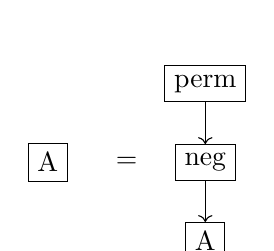
\begin{tikzpicture}
    \node[draw=black] (A) at (-2,-1) {A};
    \node[draw=black] (D1) at (0,0) {perm};
    \node[draw=black] (E1) at (0,-1) {neg};
    \node[draw=black] (F1) at (0,-2) {A};
    \node (eq) at (-1, -1) {$=$};
    \path [->] (D1) edge (E1);
    \path [->] (E1) edge (F1);
  \end{tikzpicture} 
}
Similarly, the parameter \lstinline|hs| is stating that $S$ is symmetric. Expanded in terms of tree diagrams
\proofstep{\lstinline!hS : \{S | μ ν = S | ν μ\}ᵀ!}{Description: The tensor \lstinline|S|
  is symmetric.}{
 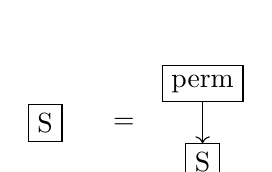
\begin{tikzpicture}
    \node[draw=black] (A) at (-2,-0.5) {S};
    \node[draw=black] (D1) at (0,0) {perm};
    \node[draw=black] (F1) at (0,-1) {S};
    \node (eq) at (-1, -0.5) {$=$};
    \path [->] (D1) edge (F1);
  \end{tikzpicture} 
}

The line \lstinline!{A | μ ν ⊗ S | μ ν = - A | μ ν ⊗ S | μ ν}ᵀ! is the statment we are trying to prove. 
In terms of tree diagrams it says that 
\begin{center}
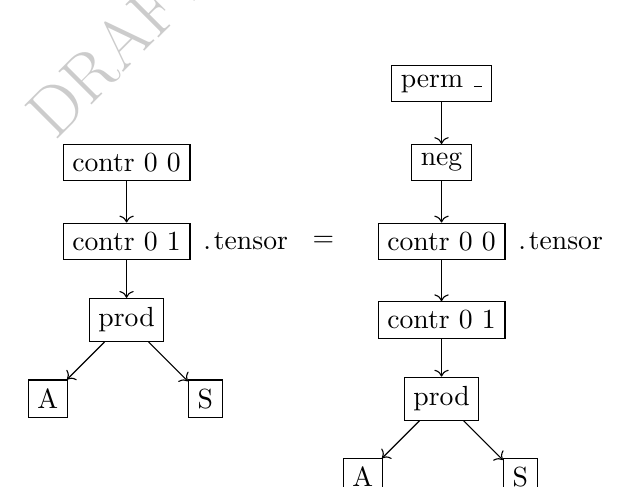
\begin{tikzpicture}
  \node (eq) at (2.5,-1) {$=$};
  \node (t1) at (1.5,-1) {\lstinline|.tensor|};
  \node (t2) at (5.5,-1) {\lstinline|.tensor|};
  \node[draw=black] (A) at (0,0) {contr 0 0};
  \node[draw=black] (B) at (0,-1) {contr 0 1};
  \node[draw=black] (C) at (0,-2) {prod};
  \node[draw=black] (D1) at (-1,-3) {A};
  \node[draw=black] (D2) at (1,-3) {S};
  \path [->] (A) edge (B);
  \path [->] (B) edge (C);
  \path [->] (C) edge (D1);
  \path [->] (C) edge (D2);
  \node[draw=black] (P') at (4,1) {perm $\_$};
  \node[draw=black] (N') at (4,0) {neg};
  \node[draw=black] (A') at (4,-1) {contr 0 0};
  \node[draw=black] (B') at (4,-2) {contr 0 1};
  \node[draw=black] (C') at (4,-3) {prod};
  \node[draw=black] (D1') at (3,-4) {A};
  \node[draw=black] (D2') at (5,-4) {S};
  \path [->] (P') edge (N');
  \path [->] (N') edge (A');
  \path [->] (A') edge (B');
  \path [->] (B') edge (C');
  \path [->] (C') edge (D1');
  \path [->] (C') edge (D2');
\end{tikzpicture}
\end{center}
The perm here actually does nothing, but is included by Lean. 

The lines of the proof in the \lstinline|conv| block are manipulations of the tensor tree on the 
LHS of the equation. The \lstinline|rw| tactic is used to rewrite the tensor tree using the various lemmas. 
We go through each step in turn. 
\proofstep{\lstinline!rw [contr_tensor_eq <| contr_tensor_eq <| prod_tensor_eq_fst <| hA]!}{
  Description: Replace the node \lstinline|A| with the RHS of \lstinline|hA|.
}{
  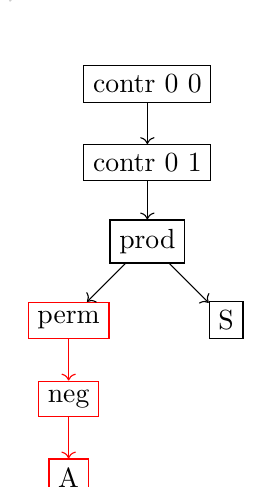
\begin{tikzpicture}
    \node[draw=black] (A) at (0,0) {contr 0 0};
    \node[draw=black] (B) at (0,-1) {contr 0 1};
    \node[draw=black] (C) at (0,-2) {prod};
    \node[draw=red] (D1) at (-1,-3) {perm};
    \node[draw=red] (E1) at (-1,-4) {neg};
    \node[draw=red] (F1) at (-1,-5) {A};
    \node[draw=black] (D2) at (1,-3) {S};
    \path [->] (A) edge (B);
    \path [->] (B) edge (C);
    \path [->] (C) edge (D1);
    \path [->, color = red] (D1) edge (E1);
    \path [->, color = red] (E1) edge (F1);
    \path [->] (C) edge (D2);
  \end{tikzpicture}
}

\proofstep{\lstinline!rw [contr_tensor_eq <| contr_tensor_eq <| prod_tensor_eq_snd <| hs]!}{
  Description: Replace the node \lstinline|S| with the RHS of \lstinline|hS|.
}{
  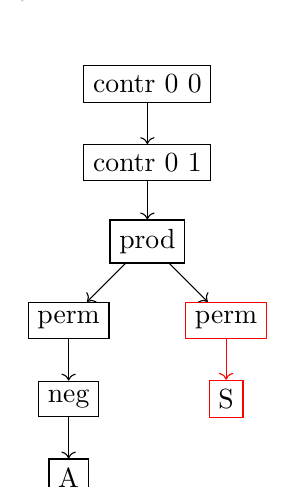
\begin{tikzpicture}
    \node[draw=black] (A) at (0,0) {contr 0 0};
    \node[draw=black] (B) at (0,-1) {contr 0 1};
    \node[draw=black] (C) at (0,-2) {prod};
    \node[draw=black] (D1) at (-1,-3) {perm};
    \node[draw=black] (E1) at (-1,-4) {neg};
    \node[draw=black] (F1) at (-1,-5) {A};
    \node[draw=red] (D2) at (1,-3) {perm};
    \node[draw=red] (F2) at (1,-4) {S};
    \path [->] (A) edge (B);
    \path [->] (B) edge (C);
    \path [->] (C) edge (D1);
    \path [->] (D1) edge (E1);
    \path [->] (E1) edge (F1);
    \path [->] (C) edge (D2);
    \path [->, color=red] (D2) edge (F2);
  \end{tikzpicture}
}

\proofstep{\lstinline!rw [contr_tensor_eq <| contr_tensor_eq <| prod_perm_left _ _ _ _]!}{
  Description: Move the left permutation through the product.
}{
  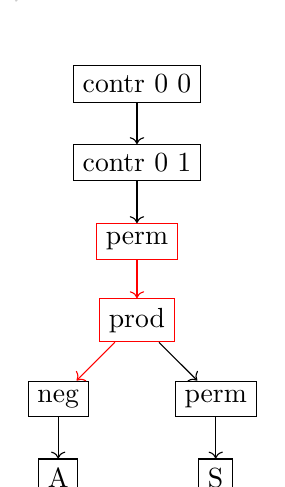
\begin{tikzpicture}
    \node[draw=black] (A) at (0,0) {contr 0 0};
    \node[draw=black] (B) at (0,-1) {contr 0 1};
    \node[draw=red] (C) at (0,-2) {perm};
    \node[draw=red] (D) at (0,-3) {prod};
    \node[draw=black] (E1) at (-1,-4) {neg};
    \node[draw=black] (F1) at (-1,-5) {A};
    \node[draw=black] (E2) at (1,-4) {perm};
    \node[draw=black] (F2) at (1,-5) {S};
    \path [->] (A) edge (B);
    \path [->] (B) edge (C);
    \path [->, color = red] (C) edge (D);
    \path [->, color = red] (D) edge (E1);
    \path [->] (E1) edge (F1);
    \path [->] (D) edge (E2);
    \path [->] (E2) edge (F2);
  \end{tikzpicture}
}

\proofstep{\lstinline!rw [contr_tensor_eq <| contr_tensor_eq <| perm_tensor_eq <| prod_perm_right _ _ _ _]!}{
  Description: Move the right permutation through the product.
}{
  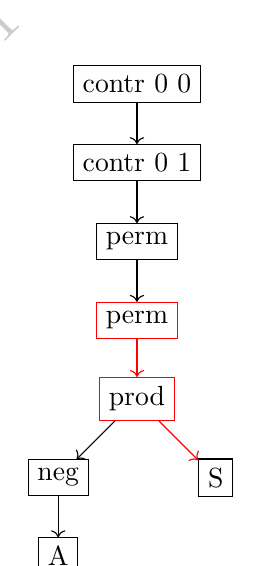
\begin{tikzpicture}
    \node[draw=black] (A) at (0,0) {contr 0 0};
    \node[draw=black] (B) at (0,-1) {contr 0 1};
    \node[draw=black] (C) at (0,-2) {perm};
    \node[draw=red] (D) at (0,-3) {perm};
    \node[draw=red] (E) at (0,-4) {prod};
    \node[draw=black] (F1) at (-1,-5) {neg};
    \node[draw=black] (G1) at (-1,-6) {A};
    \node[draw=black] (F2) at (1,-5) {S};
    \path [->] (A) edge (B);
    \path [->] (B) edge (C);
    \path [->] (C) edge (D);
    \path [->, color = red] (D) edge (E);
    \path [->] (E) edge (F1);
    \path [->, color = red] (E) edge (F2);
    \path [->] (F1) edge (G1);
  \end{tikzpicture}
}

\proofstep{\lstinline!rw [contr_tensor_eq <| contr_tensor_eq <| perm_perm _ _ _]!}{
  Description: Combine the two permutations (using functoriality).
}{
  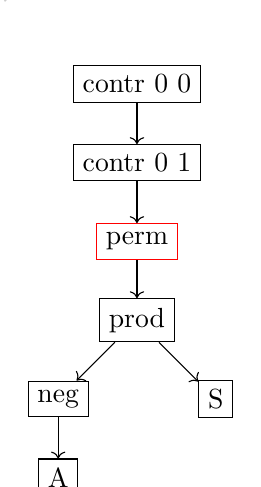
\begin{tikzpicture}
    \node[draw=black] (A) at (0,0) {contr 0 0};
    \node[draw=black] (B) at (0,-1) {contr 0 1};
    \node[draw=red] (C) at (0,-2) {perm};
    \node[draw=black] (D) at (0,-3) {prod};
    \node[draw=black] (E1) at (-1,-4) {neg};
    \node[draw=black] (F1) at (-1,-5) {A};
    \node[draw=black] (E2) at (1,-4) {S};
    \path [->] (A) edge (B);
    \path [->] (B) edge (C);
    \path [->] (C) edge (D);
    \path [->] (D) edge (E1);
    \path [->] (D) edge (E2);
    \path [->] (E1) edge (F1);
  \end{tikzpicture}
}

\proofstep{\lstinline!rw [contr_tensor_eq <| perm_contr_congr 1 2]!}{
  Description: Move the permutation through the contraction. And simplify the contraction 
  indices to \lstinline|1| and \lstinline|2| (Lean will check if this is correct).
}{
  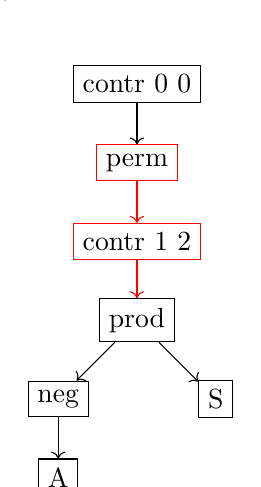
\begin{tikzpicture}
    \node[draw=black] (A) at (0,0) {contr 0 0};
    \node[draw=red] (B) at (0,-1) {perm};
    \node[draw=red] (C) at (0,-2) {contr 1 2};
    \node[draw=black] (D) at (0,-3) {prod};
    \node[draw=black] (E1) at (-1,-4) {neg};
    \node[draw=black] (F1) at (-1,-5) {A};
    \node[draw=black] (E2) at (1,-4) {S};
    \path [->] (A) edge (B);
    \path [->, color = red] (B) edge (C);
    \path [->, color = red] (C) edge (D);
    \path [->] (D) edge (E1);
    \path [->] (D) edge (E2);
    \path [->] (E1) edge (F1);
  \end{tikzpicture}
}

\proofstep{\lstinline!rw [perm_contr_congr 0 0]!}{
  Description: Move the permutation through the contraction. And simplify the contraction 
  indices to \lstinline|0| and \lstinline|0| (Lean will check if this is correct).
}{
  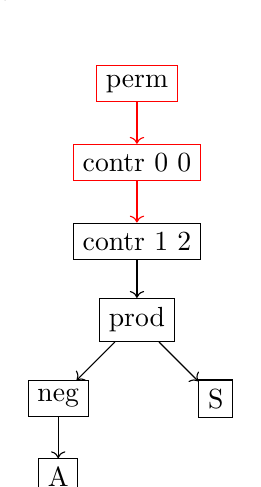
\begin{tikzpicture}
    \node[draw=red] (A) at (0,0) {perm};
    \node[draw=red] (B) at (0,-1) {contr 0 0};
    \node[draw=black] (C) at (0,-2) {contr 1 2};
    \node[draw=black] (D) at (0,-3) {prod};
    \node[draw=black] (E1) at (-1,-4) {neg};
    \node[draw=black] (F1) at (-1,-5) {A};
    \node[draw=black] (E2) at (1,-4) {S};
    \path [->, color = red] (A) edge (B);
    \path [->, color = red] (B) edge (C);
    \path [->] (C) edge (D);
    \path [->] (D) edge (E1);
    \path [->] (D) edge (E2);
    \path [->] (E1) edge (F1);
  \end{tikzpicture}
}

\proofstep{\lstinline!rw [perm_tensor_eq <| contr_contr _ _ _]!}{
  Description: Swap the two contractions. This introduces a permutation.
}{
  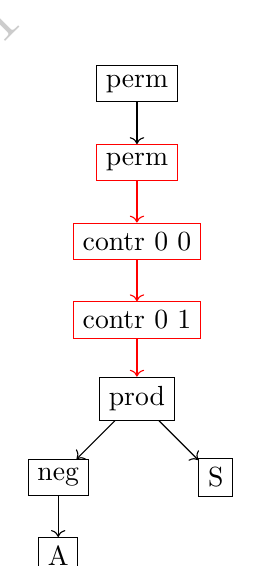
\begin{tikzpicture}
    \node[draw=black] (A) at (0,0) {perm};
    \node[draw=red] (A') at (0,-1) {perm};
    \node[draw=red] (B) at (0,-2) {contr 0 0};
    \node[draw=red] (C) at (0,-3) {contr 0 1};
    \node[draw=black] (D) at (0,-4) {prod};
    \node[draw=black] (E1) at (-1,-5) {neg};
    \node[draw=black] (F1) at (-1,-6) {A};
    \node[draw=black] (E2) at (1,-5) {S};
    \path [->] (A) edge (A');
    \path [->, color = red] (A') edge (B);
    \path [->, color = red] (B) edge (C);
    \path [->, color = red] (C) edge (D);
    \path [->] (D) edge (E1);
    \path [->] (D) edge (E2);
    \path [->] (E1) edge (F1);
  \end{tikzpicture}
}

\proofstep{\lstinline!rw [perm_perm]!}{
  Description: Combine the two permutations.
}{
  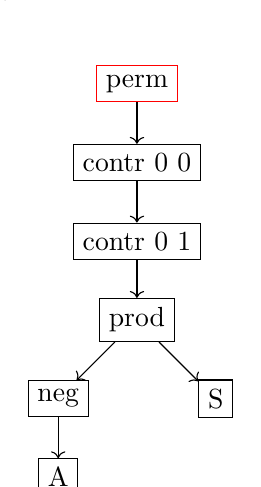
\begin{tikzpicture}
    \node[draw=red] (A) at (0,0) {perm};
    \node[draw=black] (B) at (0,-1) {contr 0 0};
    \node[draw=black] (C) at (0,-2) {contr 0 1};
    \node[draw=black] (D) at (0,-3) {prod};
    \node[draw=black] (E1) at (-1,-4) {neg};
    \node[draw=black] (F1) at (-1,-5) {A};
    \node[draw=black] (E2) at (1,-4) {S};
    \path [->] (A) edge (B);
    \path [->] (B) edge (C);
    \path [->] (C) edge (D);
    \path [->] (D) edge (E1);
    \path [->] (D) edge (E2);
    \path [->] (E1) edge (F1);
  \end{tikzpicture}
}

\proofstep{\lstinline!rw [perm_tensor_eq <| contr_tensor_eq <| contr_tensor_eq <| neg_fst_prod _ _]!}{
  Description: Move the negation through the product.
}{
  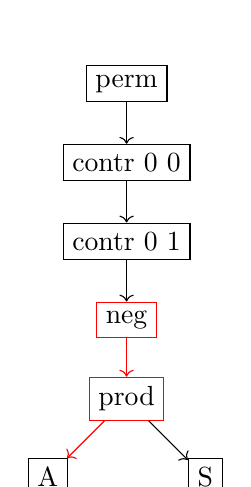
\begin{tikzpicture}
    \node[draw=black] (A) at (0,0) {perm};
    \node[draw=black] (B) at (0,-1) {contr 0 0};
    \node[draw=black] (C) at (0,-2) {contr 0 1};
    \node[draw=red] (D) at (0,-3) {neg};
    \node[draw=red] (E) at (0,-4) {prod};
    \node[draw=black] (F1) at (-1,-5) {A};
    \node[draw=black] (F2) at (1,-5) {S};
    \path [->] (A) edge (B);
    \path [->] (B) edge (C);
    \path [->] (C) edge (D);
    \path [->, color = red] (D) edge (E);
    \path [->, color = red] (E) edge (F1);
    \path [->] (E) edge (F2);
  \end{tikzpicture}
}

\proofstep{\lstinline!rw [perm_tensor_eq <| contr_tensor_eq <| neg_contr _]!}{
  Description: Move the negation through the first contraction.
}{
  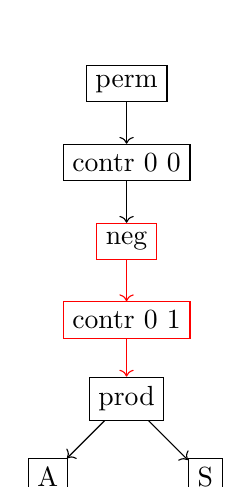
\begin{tikzpicture}
    \node[draw=black] (A) at (0,0) {perm};
    \node[draw=black] (B) at (0,-1) {contr 0 0};
    \node[draw=red] (C) at (0,-2) {neg};
    \node[draw=red] (D) at (0,-3) {contr 0 1};
    \node[draw=black] (E) at (0,-4) {prod};
    \node[draw=black] (F1) at (-1,-5) {A};
    \node[draw=black] (F2) at (1,-5) {S};
    \path [->] (A) edge (B);
    \path [->] (B) edge (C);
    \path [->, color = red] (C) edge (D);
    \path [->, color = red] (D) edge (E);
    \path [->] (E) edge (F1);
    \path [->] (E) edge (F2);
  \end{tikzpicture}
}

\proofstep{\lstinline!rw [perm_tensor_eq <| neg_contr _]!}{
  Description: Move the negation through the second contraction.
}{
  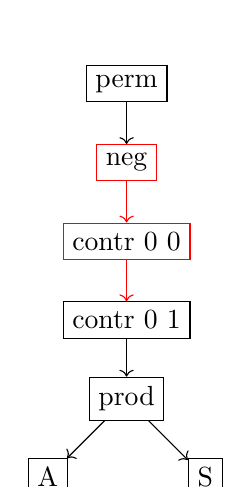
\begin{tikzpicture}
    \node[draw=black] (A) at (0,0) {perm};
    \node[draw=red] (B) at (0,-1) {neg};
    \node[draw=red] (C) at (0,-2) {contr 0 0};
    \node[draw=black] (D) at (0,-3) {contr 0 1};
    \node[draw=black] (E) at (0,-4) {prod};
    \node[draw=black] (F1) at (-1,-5) {A};
    \node[draw=black] (F2) at (1,-5) {S};
    \path [->] (A) edge (B);
    \path [->, color = red] (B) edge (C);
    \path [->, color = red] (C) edge (D);
    \path [->] (D) edge (E);
    \path [->] (E) edge (F1);
    \path [->] (E) edge (F2);
  \end{tikzpicture}
}

The remainder of the proof \lstinline|apply perm_congr _ rfl| and \lstinline|decide| that the 
tensor trees on the LHS and RHS are actually equal.
\subsection{Example 2: Pauli matrices and bispinors} \label{sec:examplePauliBispinor}

Using the formlism we have set up thus far it is possible to define Pauli matrices and bispinors 
as complex Lorentz tensors.
 
The pauli matrices appear in HepLean as follows 
\begin{code}
/-- The Pauli matrices as the complex Lorentz tensor `σ^μ^α^{dot β}`. -/
def pauliContr := {PauliMatrix.asConsTensor | ν α β}ᵀ.tensor

/-- The Pauli matrices as the complex Lorentz tensor `σ_μ^α^{dot β}`. -/
def pauliCo := {η' | μ ν ⊗ pauliContr | ν α β}ᵀ.tensor

/-- The Pauli matrices as the complex Lorentz tensor `σ_μ_α_{dot β}`. -/
def pauliCoDown := {pauliCo | μ α β ⊗ εL' | α α' ⊗ εR' | β β'}ᵀ.tensor

/-- The Pauli matrices as the complex Lorentz tensor `σ^μ_α_{dot β}`. -/
def pauliContrDown := {pauliContr | μ α β ⊗ εL' | α α' ⊗ εR' | β β'}ᵀ.tensor
\end{code}
The first of these definitions depends on \lstinline|PauliMatrix.asConsTensor| which is defined as 
using an explcit basis expansion. 

In these expressions we have the appearence of metrics \lstinline|η'| is the metric usually written as 
$\eta_{\mu \nu}$, \js{etc.}

With these we can define bispinors 
\begin{code}
/-- A bispinor `pᵃᵃ` created from a lorentz vector `p^μ`. -/
def contrBispinorUp (p : complexContr) :=
  {pauliCo | μ α β ⊗ p | μ}ᵀ.tensor

/-- A bispinor `pₐₐ` created from a lorentz vector `p^μ`. -/
def contrBispinorDown (p : complexContr) :=
  {εL' | α α' ⊗ εR' | β β' ⊗ contrBispinorUp p | α β}ᵀ.tensor

/-- A bispinor `pᵃᵃ` created from a lorentz vector `p_μ`. -/
def coBispinorUp (p : complexCo) := {pauliContr | μ α β ⊗ p | μ}ᵀ.tensor

/-- A bispinor `pₐₐ` created from a lorentz vector `p_μ`. -/
def coBispinorDown (p : complexCo) :=
  {εL' | α α' ⊗ εR' | β β' ⊗ coBispinorUp p | α β}ᵀ.tensor
\end{code}
Here \lstinline|complexContr| and \lstinline|complexCo| are complex contravariant and covariant Lorentz vectors.
Lean knows to treat these as tensors when they appear in tensor expressions. 


Using these definitions we can start to prove results about the pauli matrices and bispinors. 
These proofs reyl on essentially the sorts of manipulations in the last section, although in some cases 
we expand tensors in terms of a basis and use rules about how the basis interacts with the operations in a tensor tree. 

Examples of things we have proven range  
\begin{code}
lemma coBispinorDown_eq_pauliContrDown_contr (p : complexCo) :
  {coBispinorDown p | α β = pauliContrDown | μ α β ⊗ p | μ}ᵀ := by
\end{code}
the proof of which is an application of associativity of the tensor product, and appropratly shuffling 
around of the contractions. 

To more complicated results such as
\begin{code}
/-- The statement that `η_{μν} σ^{μ α dot β} σ^{ν α' dot β'} = 2 ε^{αα'} ε^{dot β dot β'}`. -/
theorem pauliCo_contr_pauliContr :
    {pauliCo | ν α β ⊗ pauliContr | ν α' β' = 2 •ₜ εL | α α' ⊗ εR | β β'}ᵀ := by
\end{code}


\section{Future work} \label{sec:future}
The scale of formalizing all results regarding index notation is a task that surpasses 
the capacity of any single individual. Inspired by the Lean community's 
blueprint projects, we have added to HepLean informal lemmas related to index notation and tensors. 
An example of such is 
\begin{code} 
informal_lemma coBispinorUp_eq_metric_contr_coBispinorDown where
  math :≈ "{coBispinorUp p | α β = εL | α α' ⊗ εR | β β' ⊗ coBispinorDown p | α' β' }ᵀ"
  proof :≈ "Expand `coBispinorDown` and use fact that metrics contract to the identity."
  deps :≈ [``coBispinorUp, ``coBispinorDown, ``leftMetric, ``rightMetric]
\end{code}
The lemmas  resource that we hope others—or even automated systems—will formalize in the future.

As demonstrated in our earlier examples, manipulating tensor expressions can involve tedious
 calculations, especially when dealing with directly with tensor trees. 
In the future, we intend to automate many of these routine steps by developing suitable tactics 
within Lean. We are optimistic that the structured nature of tensor trees will lend itself well to 
such automation, thereby streamlining computations and enhancing the efficiency of formal proofs
involving index notation and tensor species.

There are two primary directions in which we can extend the concepts presented in this work. 
First, we could incorporate the spinor-helicity formalism, which is used in the study of scattering 
amplitudes. Second, we could extend our approach to encompass tensor \emph{fields}, their derivatives
etc. We do not anticipate any insurmountable challenges in pursuing these extensions. 
They represent promising avenues for future research and have the potential to significantly enhance
the utility of formal methods in physics.
\bibliographystyle{unsrturl}
\begin{spacing}{0.5}
\bibliography{MyBib}
\end{spacing}


%%%%%%%%%%%%%%
\end{document}
